% --------------------------------------------------------------------------
% Version 3.0
% This template is available on the sites:
% https://www.overleaf.com/read/rpkkfchcnbsc
% https://www.overleaf.com/latex/templates/itmo-beamer-theme/fpttrgnmqwsb
% https://github.com/AlexZabashta/ITMO-Beamer-theme
% --------------------------------------------------------------------------

% Attention!!!
% This document was created only as an example of using ITMO beamer styling.
% Don't use it as a Latex or beamer tutorial!
% Check out the capabilities of Latex and beamer (at least basic) independently.


\documentclass[aspectratio=169]{beamer}
\usepackage{ITMOtheme}
\usepackage{dirtytalk}
\usepackage{hyperref}


% Use this package to automatically format references.
% \usepackage[style=mla]{biblatex}
% \addbibresource{references.bib}


%\titlegraphic{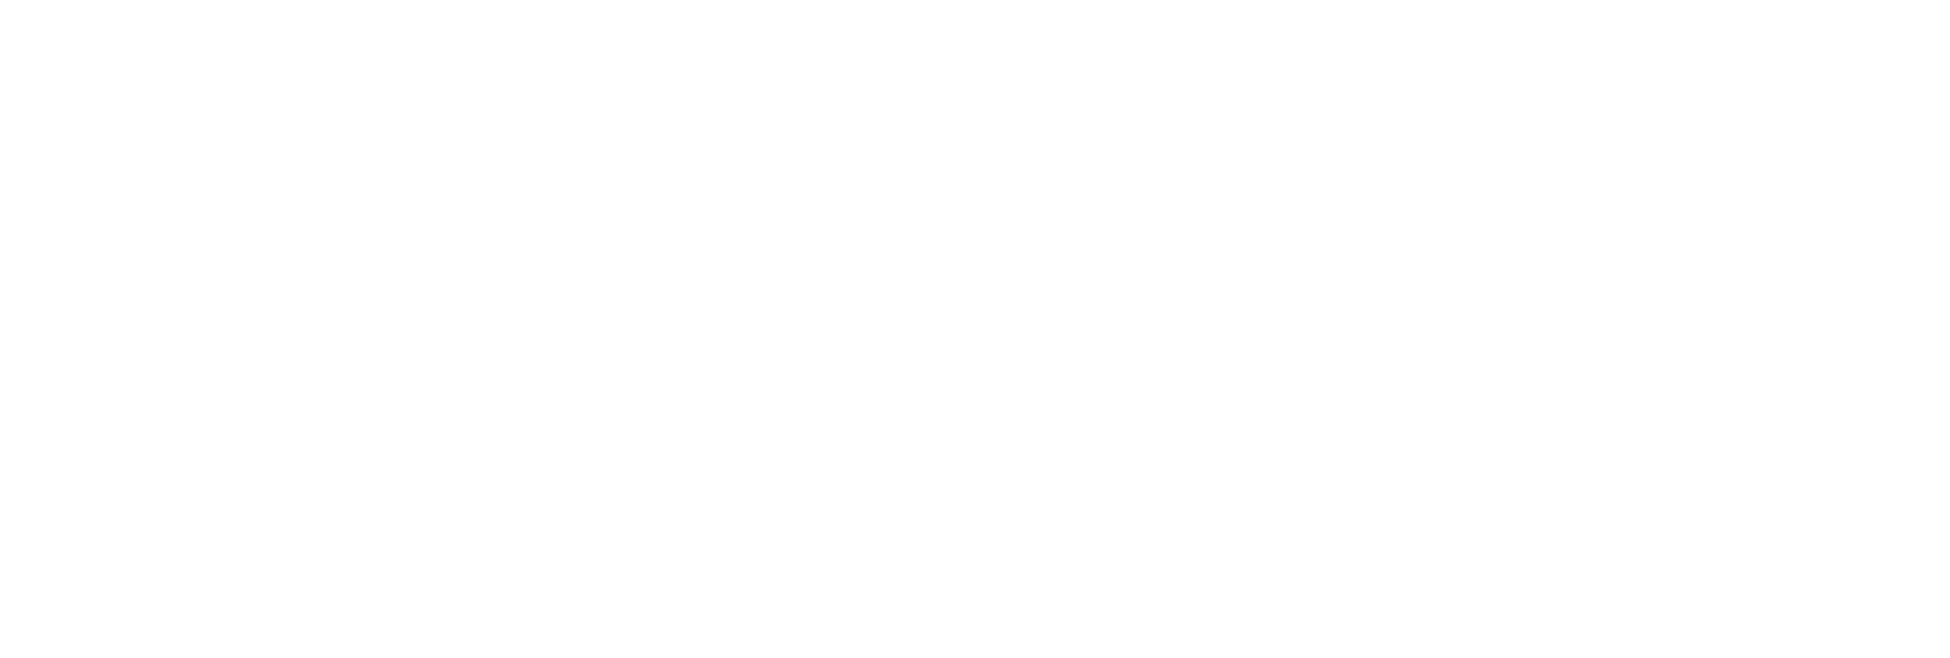
\includegraphics[width=0.2\textwidth]{itmo/logo_basic_english_white.pdf}}

% The fields 'title', 'author', 'subject', 'keywords' are used to generate a PDF document.
% It is recommended that you fill them in, even if you are creating your title slide manually.

% use \title[short title]{full title}
\title[MRAM Pros \& Cons]{MRAM: La promesa Electromagnetica}

%\subtitle[short subtitle]{long subtitle}

\author[Pachon D.]{David Pachon \\ Sergio Montoya}

%\institute[short institute]{long institute}

\where{Bogota, Colombia}
\date{\today}


\subject{example}
\keywords{ITMO University, LaTex teamplate, beamer}



\begin{document}


% [plain] - modifier to create a blank slide (without bottom bar).
% Ideal for creating the first (title) and last slide with a polygonal background,
% or for transitional slides between chapters or slides with a table of contents.

% \titlepage - command for automatic generation of title slide content.

\begin{frame}[plain]
    \titlepage
\end{frame}

% You can use custom title, if you want.
% Or you can you modify the .sty file.


%\begin{frame}[plain]
	%\itmobackgroundsnakes{
	%\vfill
		%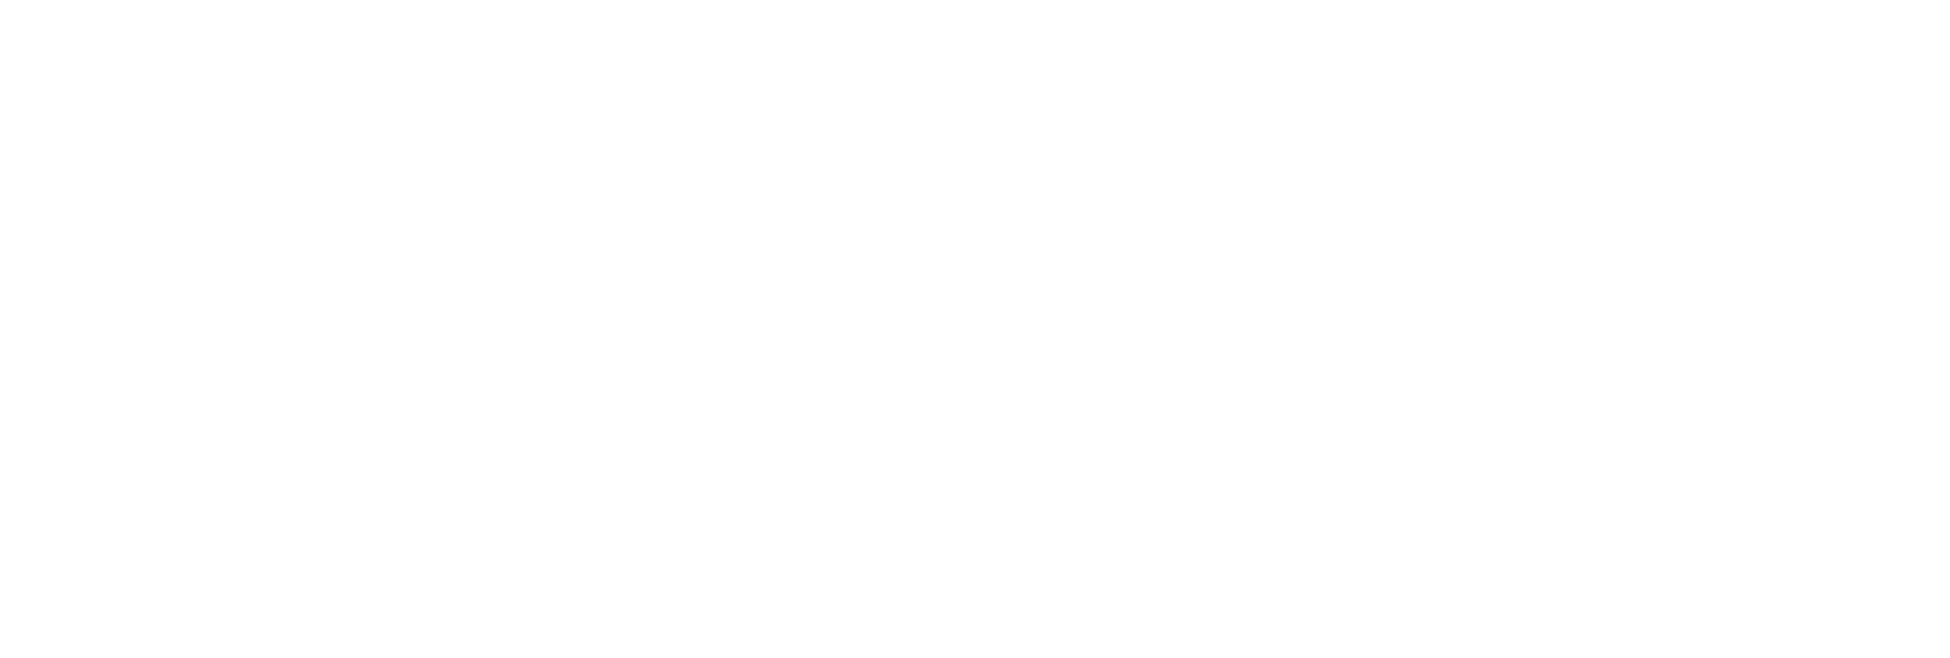
\includegraphics[width=0.2\textwidth]{itmo/logo_basic_english_white.pdf}
	%\vfill
		%\usebeamerfont{title}{  \inserttitle\par} 
	%\vfill
		%Custom title slide
	%\vfill
		%\insertauthor\par
	%\vfill
		%\insertplace  \;  \insertdate
%}
%\end{frame}


% Avoid making a table of contents in short presentations.
% Transitions between chapters are best done manually.

\begin{frame}{Imagina\ldots}
    Imagina que estás queriendo conseguir el récord mundial de cálculo de dígitos de Pi (que actualmente se encuentra en aproximadamente $300.000.000.000.000$). Entonces, el espacio que ocuparía, asumiendo que usas un \textit{nibble} (4 bits) para almacenar cada dígito, sería de unos \textbf{150 terabytes}.¿Donde podrias guardar tanta información?
\end{frame}

\begin{frame}{SOTA: HD}
    \begin{center}
    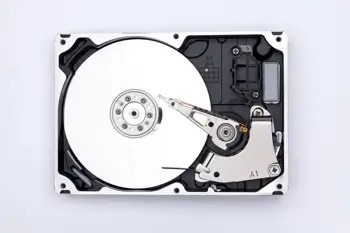
\includegraphics[scale=.75]{fig/hard-disk-drive.jpeg}
    \end{center}
\end{frame}


\begin{frame}{SOTA: DRAM}
    \begin{center}
    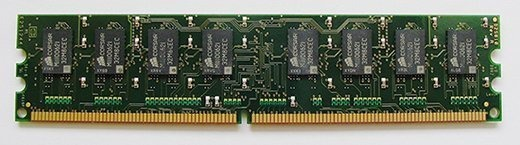
\includegraphics[scale=.65]{fig/dram_1.jpeg}
    \end{center}
\end{frame}

\begin{frame}{¿Por que no se usa una sola?}
    \begin{itemize}
        \item Velocidad de un SSD (Mucho mas rapido que un HD): 50 microsegundos
        \item Velocidad de un DRAM: 17 nanosegundos (3000 veces mas rapido)
        \item DRAM es volatil
    \end{itemize}

    De ahi nace una propuesta de solución: MRAM
\end{frame}

\begin{frame}{¿Qué es una MTJ (Magnetic Tunnel Junction)?}
Capa de barrera (generalmente de óxido de magnesio, MgO): Es una barrera delgada (~1 nm) que permite el tunelamiento cuántico de electrones.
\end{frame}

\begin{frame}{¿Qué es una MTJ (Magnetic Tunnel Junction)?}
\begin{columns}[c] 
\column{.45\textwidth}{
La resistencia eléctrica de la MTJ depende de la relación entre las direcciones de magnetización de las dos capas ferromagnéticas:

Paralela $\to$ baja resistencia (estado lógico 0).

Antiparalela $\to$ alta resistencia (estado lógico 1).

Este fenómeno se conoce como magnetorresistencia de túnel (TMR).
}

\column{.45\textwidth}{
    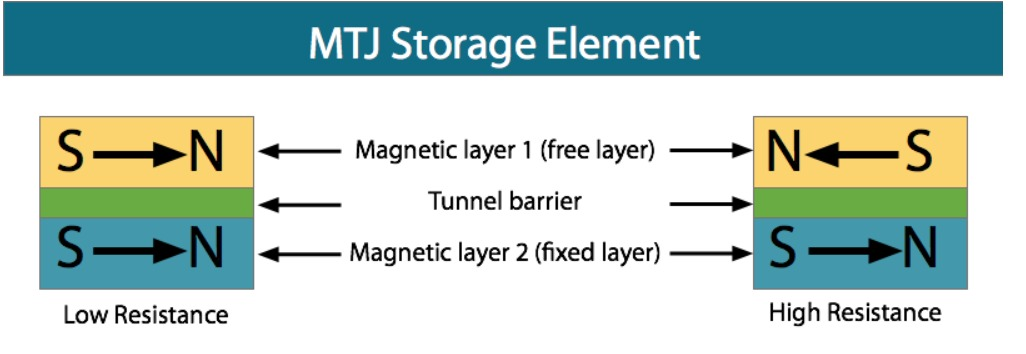
\includegraphics[scale=.25]{fig/mtj.jpeg}
}

\end{columns}
\end{frame}

\begin{frame}{Toggle MRAM}
    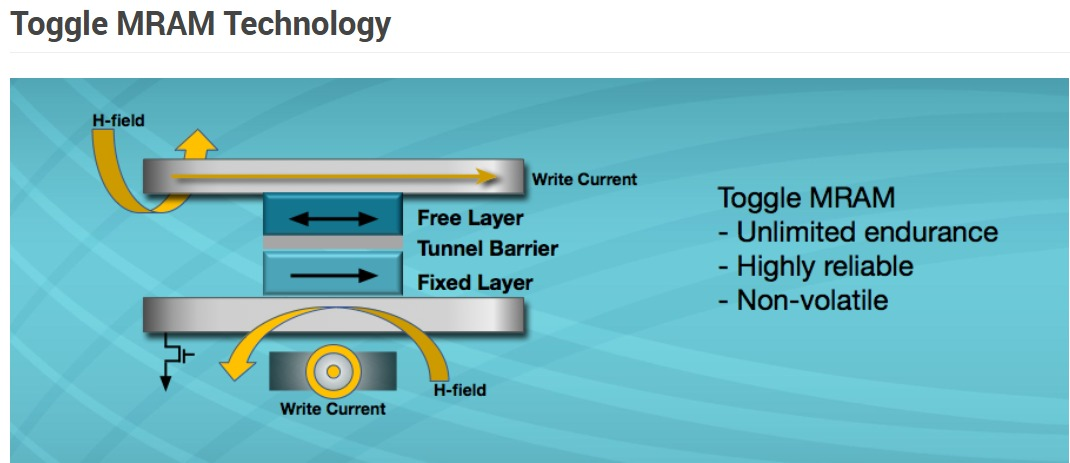
\includegraphics[scale=.45]{fig/mram_1.jpeg}
\end{frame}

\begin{frame}{spin dependent tunnel junction}
    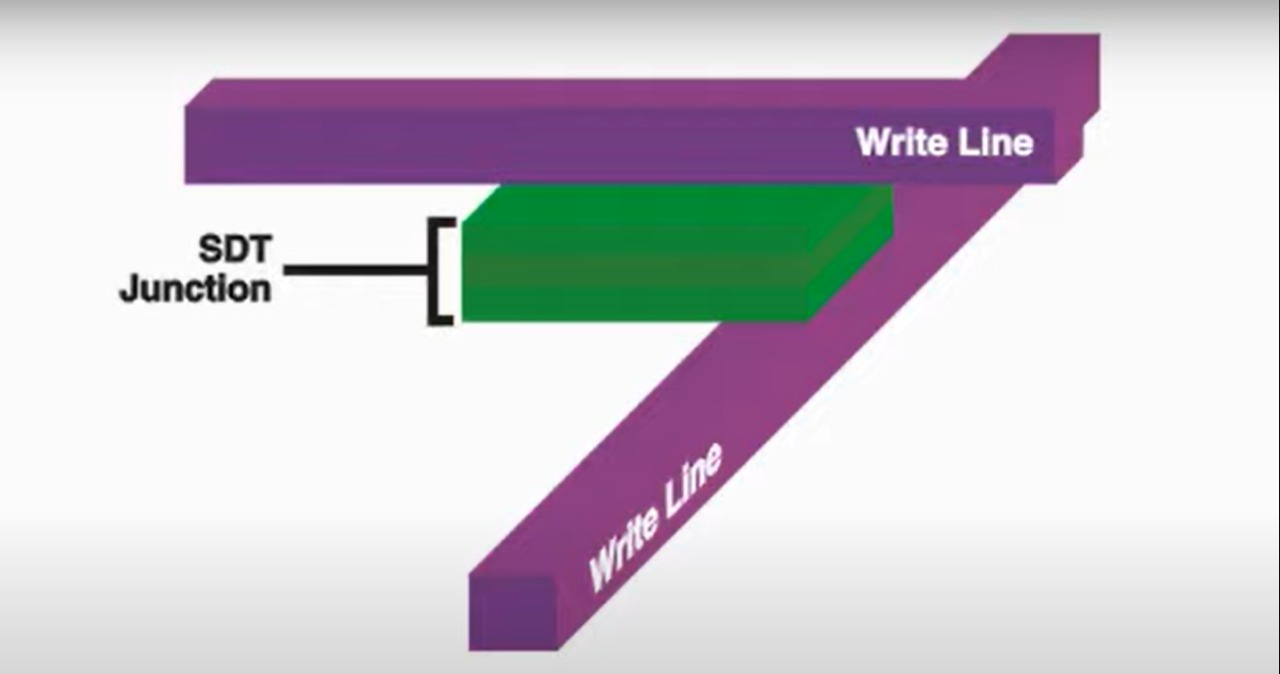
\includegraphics[scale=.45]{fig/sdt_1.jpeg}
\end{frame}

\begin{frame}{MRAM}
    \begin{columns}
        \column{.45\textwidth}{
Corriente por la word line $\to$ genera un campo magnético en una dirección (por ejemplo, horizontal).

Corriente por la bit line $\to$ genera un campo magnético en la dirección perpendicular (por ejemplo, vertical).
        }
        \column{.45\textwidth}{
                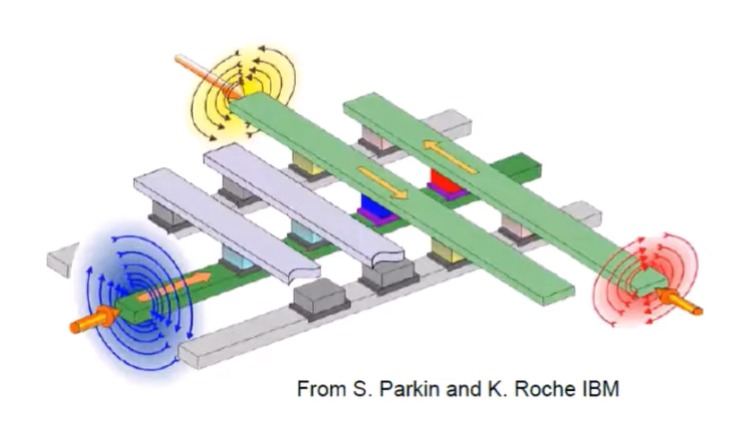
\includegraphics[scale=.25]{fig/mram_2.jpeg}
        }
    \end{columns}
\end{frame}

\begin{frame}{MRAM}
    \begin{columns}
        \column{.45\textwidth}{
            Solo la capa libre cambia su magnetización porque está diseñada para ser sensible a los campos magnéticos. En cambio, la capa fija está \say{anclada} mediante una capa antiferromagnética y materiales más resistentes al cambio, por lo que permanece inalterada.
        }
        \column{.45\textwidth}{
                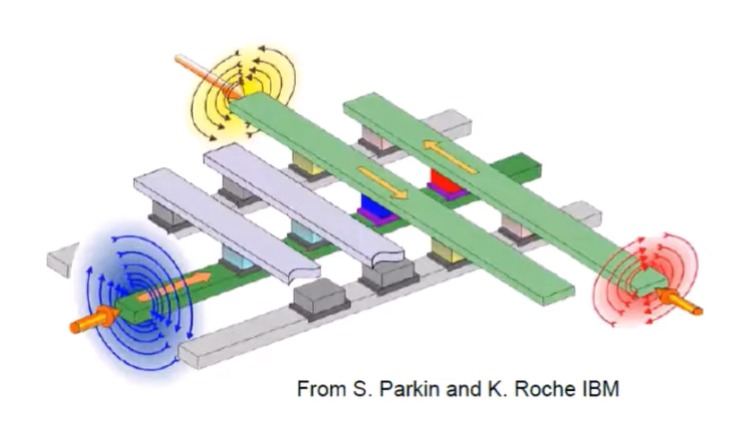
\includegraphics[scale=.25]{fig/mram_2.jpeg}
        }
    \end{columns}
\end{frame}

\begin{frame}{Lectura de un bit en MRAM}
Se aplica un voltaje de lectura entre la bit line y la tierra.
La corriente atraviesa la MTJ (Magnetic Tunnel Junction).
Se mide la corriente resultante.
Usando la ley de Ohm 
    \[R = \frac{V}{I}\]
Se calcula la resistencia de la MTJ.
Según el valor de resistencia:

Baja resistencia $\to$ Estados paralelos $\to$ bit = 0

Alta resistencia $\to$ Estados antiparalelos $\to$ bit = 1

La lectura no cambia el estado del bit.

    \alert{La corriente de lectura es muy pequeña para no afectar la magnetización.}
\end{frame}


\begin{frame}[plain]
    \itmobackgroundsnakes{
        \vfill
        \Huge{The End}
        \vfill
    }
\end{frame}


\begin{frame}[noframenumbering]
    \frametitle{References}
    {\footnotesize
    \begin{enumerate}
        \item \textit{Dynamic Random Acess Memory (DRAM) Explained | 'All About Semiconductor' by Samsung Semiconductor}. \\ 
            \url{https://youtu.be/_pdwsakYhMk?feature=shared}

        \item \textit{How does Computer Memory Work?}. \\
            \url{https://youtu.be/7J7X7aZvMXQ?feature=shared}

        \item \textit{What Is MRAM?}. \\ 
            \url{https://youtu.be/VRJ7xYPMfGA?si=rT4iHyEM_GpyUh2x}
    
        \item \textit{Prof. Tiffany Santos: Spins, Bits \& Flips: Essentials for a High-Density MRAM}. \\ 
            \url{https://youtu.be/GyjPeqqWeKA?feature=shared}

        \item Libro: Scott, J. C. \textit{But How Do It Know? - The Basic Principles of Computers for Everyone}. \\ 
            \url{https://www.amazon.com/But-How-Know-Principles-Computers/dp/0615303765}
    \end{enumerate}}
\end{frame}


\end{document}
